% Digital Logic Report Template
% Created: 2020-01-10, John Miller

%==========================================================
%=========== Document Setup  ==============================

% Formatting defined by class file
\documentclass[11pt]{article}

% ---- Document formatting ----
\usepackage[margin=1in]{geometry}	% Narrower margins
\usepackage{booktabs}				% Nice formatting of tables
\usepackage{graphicx}				% Ability to include graphics

%\setlength\parindent{0pt}	% Do not indent first line of paragraphs 
\usepackage[parfill]{parskip}		% Line space b/w paragraphs
%	parfill option prevents last line of pgrph from being fully justified

% Parskip package adds too much space around titles, fix with this
\RequirePackage{titlesec}
\titlespacing\section{0pt}{8pt plus 4pt minus 2pt}{3pt plus 2pt minus 2pt}
\titlespacing\subsection{0pt}{4pt plus 4pt minus 2pt}{-2pt plus 2pt minus 2pt}
\titlespacing\subsubsection{0pt}{2pt plus 4pt minus 2pt}{-6pt plus 2pt minus 2pt}

% ---- Hyperlinks ----
\usepackage[colorlinks=true,urlcolor=blue]{hyperref}	% For URL's. Automatically links internal references.

% ---- Code listings ----
\usepackage{listings} 					% Nice code layout and inclusion
\usepackage[usenames,dvipsnames]{xcolor}	% Colors (needs to be defined before using colors)

% Define custom colors for listings
\definecolor{listinggray}{gray}{0.98}		% Listings background color
\definecolor{rulegray}{gray}{0.7}			% Listings rule/frame color

% Style for Verilog
\lstdefinestyle{Verilog}{
	language=Verilog,					% Verilog
	backgroundcolor=\color{listinggray},	% light gray background
	rulecolor=\color{blue}, 			% blue frame lines
	frame=tb,							% lines above & below
	linewidth=\columnwidth, 			% set line width
	basicstyle=\small\ttfamily,	% basic font style that is used for the code	
	breaklines=true, 					% allow breaking across columns/pages
	tabsize=3,							% set tab size
	commentstyle=\color{gray},	% comments in italic 
	stringstyle=\upshape,				% strings are printed in normal font
	showspaces=false,					% don't underscore spaces
}

% How to use: \Verilog[listing_options]{file}
\newcommand{\Verilog}[2][]{%
	\lstinputlisting[style=Verilog,#1]{#2}
}




%======================================================
%=========== Body  ====================================
\begin{document}

\title{ELC 2137 Lab 1: Lab Title}
\author{Sam Jeffrey}

\maketitle


\section*{Summary}



\section*{Q\&A}


\begin{enumerate}
\item  What is your GitHub user name?
 
Awnser: My user name is samjeffrey1

\item  What  LaTeX  environment  produces  a  bulleted(non-numbered) list?

Awnser: The itemize environment produces bulleted lists.

\item  Write  the  equationy(t) = 1/2 $e^t$ using  La-TeX equation formatting.

Awnser: 
\begin{equation}
	y(t) = \frac{1}{2}e^t
\end{equation}

\item  What is the shortcut key for compiling your La-TeX document?

Awnser: F5

\end{enumerate}


\section*{Results}


\begin{figure}[ht]\centering
	\begin{tabular}{c|c|c}
		\toprule
		Binary & Hex & Decimal \\
		\midrule
		0000 & 0 & 0 \\
		0010 & 2 & 2 \\
		0100 & 4 & 4 \\
		0110 & 6 & 6 \\
		1000 & 8 & 8 \\
		1010 & A & 10 \\
		\bottomrule
	\end{tabular} 
	\caption{Converting between binary, Hex and Decimal}
\label{tbl:example_table}
\end{figure}

\begin{figure}[ht]\centering
	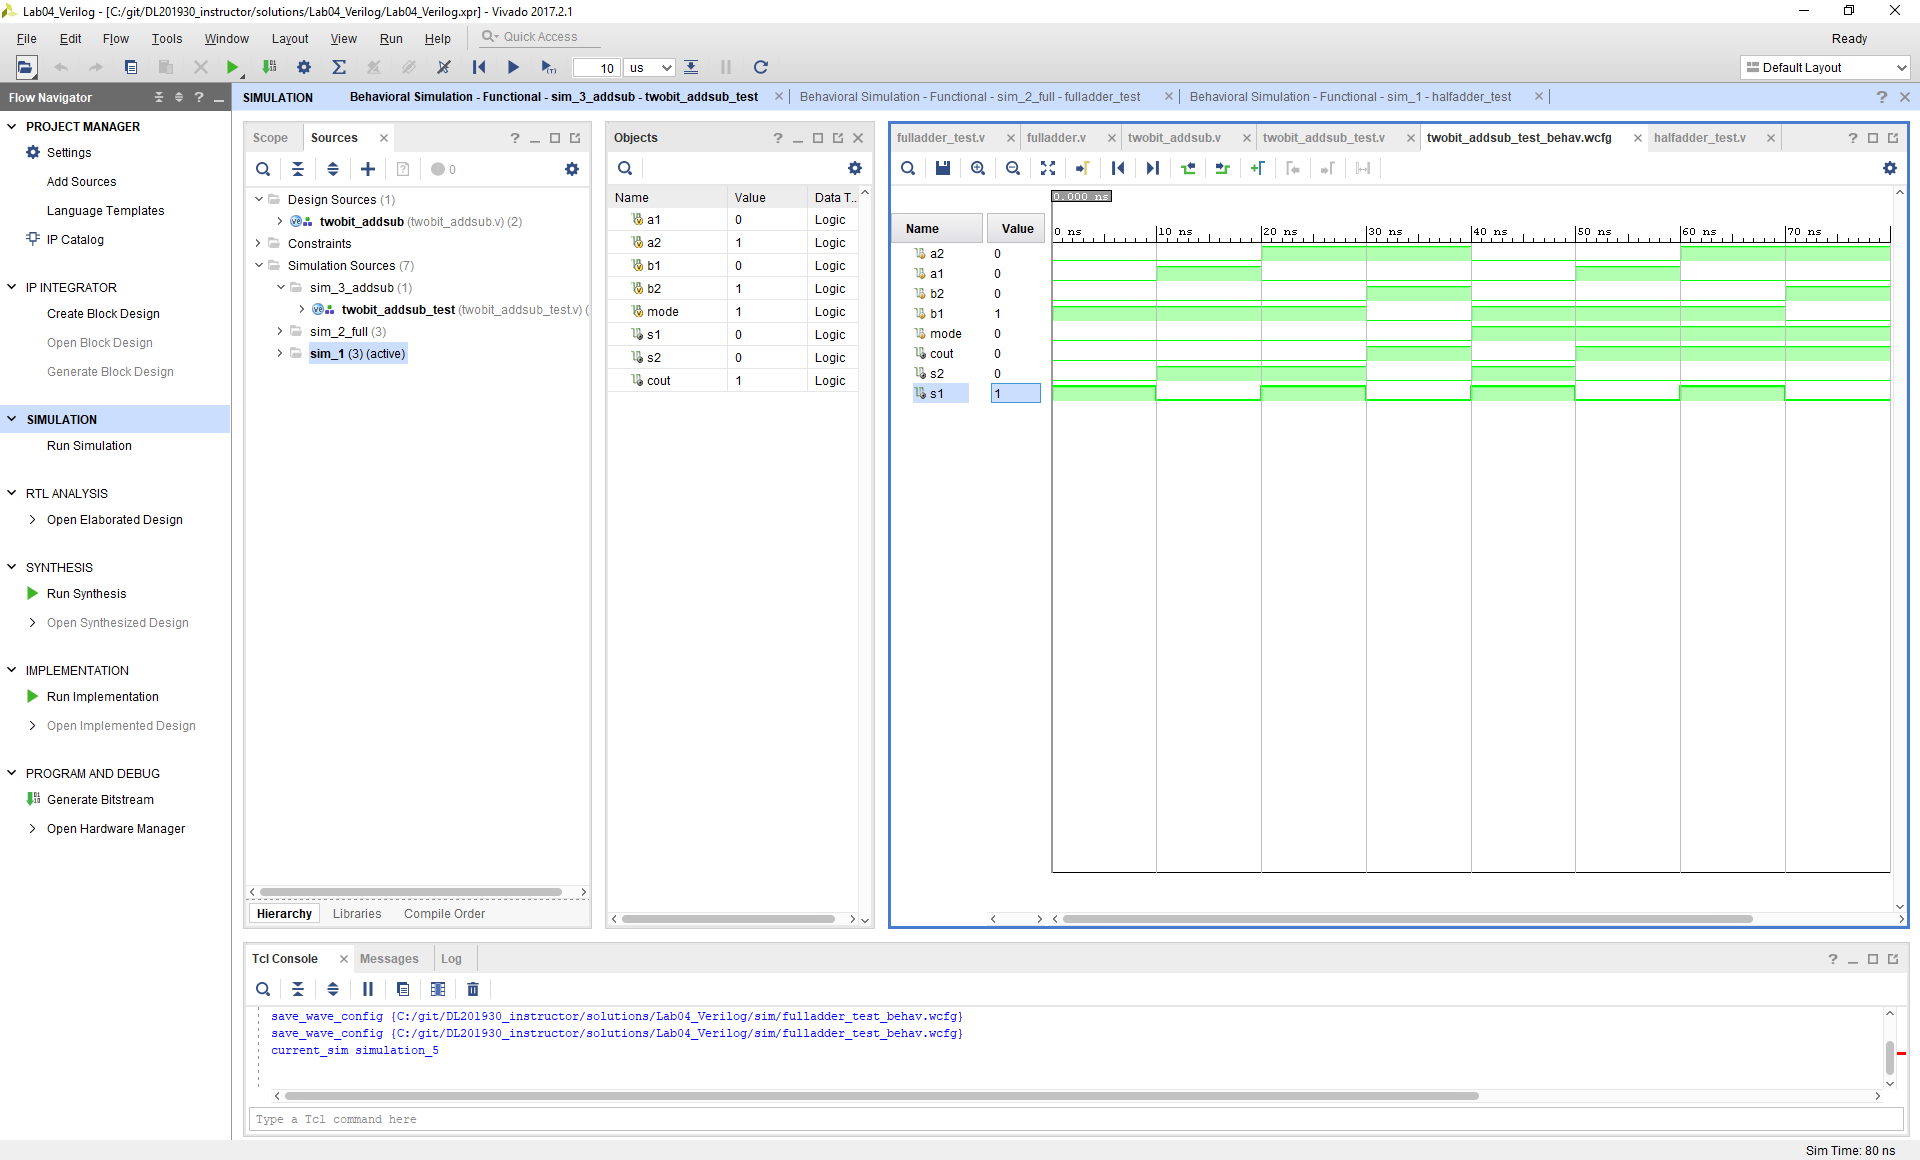
\includegraphics[width=1\textwidth,trim=18.5cm 15.75cm .5cm 4.5cm,clip]{lab1_example_screenshot.PNG}
	\caption{Simulation waveform}
	\label{fig:another_image}          % label must be after caption
\end{figure}


\section*{Code}

\Verilog[caption=File-included Verilog code example,label=code:file\_ex]{example\_code.sv}


\end{document}
